\documentclass{scrartcl}
\usepackage[utf8]{inputenc}
\usepackage{enumitem}
\usepackage{graphicx}
\usepackage{multirow,tabularx}
\usepackage{etoolbox}
\usepackage{indentfirst}

\newcounter{rowcnt}
\newcommand\rownum{\ifnumequal{\value{rowcnt}}{0}{No.}{\therowcnt.}\refstepcounter{rowcnt}}
\AtEndEnvironment{tabularx}{\setcounter{rowcnt}{0}}

\title{True Randomness using the Randomness in Physical Phenomenon}
\subtitle{Interim Report}
\author{Kanchana Senadheera}
\date{20 January 2019}

\begin{document}

\maketitle

\section*{Abstract}
Random numbers or specifically referred to as Random Bit Streams, play a vital role in a number of disciplines. However, due to the nature of modern day computers, the randomness generated by them are well below from the truly random nature. This study is an attempt to discover the possibility of making use of the environmental randomness into the computers, so that they generate better randomness.
\par This report is compiled to summarize the present progress of the work that needs to be undertaken. First section outlines the work items that were initially planned during the proposal stage and how those have been broken down into measurable work items. Second section summarizes the progress in both tabular and graphical form, with the help of tools such as Gantt Charts. Then the report is concluded with a critical review on the progress attained to the date.

\section{Introduction}
\textbf{Random Numbers} or \textbf{Random Bits} (mostly known in computing) is an essential component in modern day information security. This is due to the fact that most of the implementations of information security, including encryption algorithms, hashing algorithms and so forth, are required to have some random bits at some point of their life cycles. Apart from that, some other disciplines including but not limited to statistics, physics, mathematical computing.
\par Randomness is defined in many different ways, taking many different aspects into consideration. Cambridge English Dictionary define randomness as "\textit{happening, done, or chosen by chance rather than according to a plan}" and "\textit{by chance, or without being chosen intentionally}"\cite{web_cambridge_def_rnd}. Here the second definition seems more appropriate to most of the modern day applications. Further, according to Oxford English Dictionary, randomness is "\textit{made, done, or happening without method or conscious decision}"\cite{web_oxford_def_rnd}. This also emphasizes on the fact that \textit{absolute lack of bias} should be a definite characteristic of randomness. 
\par All modern computers are finite state machines; as in, they change their state when they read inputs. So, it is obvious that, the state of the machine is entirely dependent on the input given. Hence it does not demonstrate true-random behavior because, it is in most of the cases possible to manipulate the inputs, so that the state machine transfers into a desired/intended state. This eliminates or degrades the requirement of \textit{absolute lack of bias}.
\par Alternative that satisfies these requirements partially, is Pseudo-Randomness. This is achieved with the help of Pseudo-Random Number Generators (PRNG). A PRNG is typically
    \begin{enumerate}
        \item A machine that has a deterministic algorithm at its core (computer program/subroutine, hardware device attached)
        \item In most cases takes random bits as input (seed)
    \end{enumerate}
\par However, most of these generators seem to fall short in front of certain requirements such as,
    \begin{itemize}
        \item Complexity requirements
        \item Volume requirements
        \item Performance requirements
    \end{itemize}
\par However, there are some phenomenon that exist in the surrounding environments, that demonstrates better randomness. This research study attempts to evaluate the feasibility of using that \textbf{Environmental Randomness} as a source to be used in modern day binary computers.

\newpage\section{Work Planned}
    \subsection{Methodology}
        The proposed methodology of the research study is as follows
        \begin{enumerate}
            \item Define and clarify between true-randomness and pseudorandomness
            \item Closely review the existing algorithms to identify their limitations
            \item Identify possible sources of Randomness and their limitations
            \item Determine the exact (still uncertain) evaluation criteria
            \item Determine the mathematical models for transformation
            \item Implement the models
            \item Evaluate the models and document the observations and conclusions
        \end{enumerate}
        
    \subsection{Work Plan based on the Methodology}
        The actual execution of the above methodology was planned according to the following work items for each stage of the methodology.
        \begin{enumerate}[ref=\theenumi]
            \item Define and clarify between true-randomness and pseudo-randomness
            \begin{enumerate}[ref=\theenumi.\theenumii]
                \item\label{def_rnd} Establishment of a definition for randomness
                \item\label{obs_fsm} Observe the nature of the behavior of a finite state machine and determine if it demonstrate any behaviors that matches the above definition
            \end{enumerate}
            
            \item Closely review the existing algorithms to identify their limitations
            \begin{enumerate}[ref=\theenumi.\theenumii]
                \item\label{id_alg} Enumerate some well-known and widely used algorithms and obtain their implementations
                \item\label{und_alg} Understand how they behave in certain critical corner cases (these cases might be general or sometimes might be specific to each algorithm)
                \item\label{alg_pro_con} Identify and enumerate their pros and cons
            \end{enumerate}
            
            \item Identify possible sources of Randomness and their limitations
            \begin{enumerate}[ref=\theenumi.\theenumii]
                \item\label{id_measures} Identify and enumerate the programmatically measurable phenomenons
                \item\label{capt_data} Capture the data correspond to those metrics over a considerably long duration
                \item\label{vis_data} Visualize the captured data to observe their patterns (if there are any)
                \item\label{filter_met} Based on the observations, filter out the metrics which are demonstrating patterns.
            \end{enumerate}
            
            \item Determine the exact (still uncertain) evaluation criteria
            \begin{enumerate}[ref=\theenumi.\theenumii]
                \item\label{id_eval} Identify and enumerate the commonly used evaluation criterion for RNGs
                \item\label{det_suit} Determine the suitability (as applicable) and choose the criterion.
            \end{enumerate}
            
            \item Determine the mathematical models for transformation
            \begin{enumerate}[ref=\theenumi.\theenumii]
                \item\label{det_requ} Determine the requirements that the output should satisfy
                \item\label{id_math_models} Identify the existing mathematical operations and models that combine operations
                \item\label{det_models_ops} Determine the models/combinations of models/new models that combines operations
            \end{enumerate}
            
            \item Implement the models
            \begin{enumerate}[ref=\theenumi.\theenumii]
                \item\label{id_lang_env} Identify suitable languages and environment
                \item\label{impl} Implement the models
            \end{enumerate}
            
            \item\label{test} Evaluate the models and document the observations and conclusions
            
            \item\label{thesis} Compile the Research Thesis
        \end{enumerate}
\newpage\section{Work Complete}
Completed work items are listed below, with references to the WBS items.
    \begin{table}[htb]
        \centering
        \begin{tabularx}{\textwidth}{ |>{\rownum}r|l|X| }
            \hline
            & WBS Item & Remarks \\ \hline
            
            & \ref{def_rnd} & Established the definition of randomness in terms of mathematics and computing \\ \hline
            
            & \ref{obs_fsm} & Observed and identified that the operations that a finite state machine executes, will not produce output that could be determined as random (according to the definition identified above) \\ \hline
            
            & \ref{id_alg} &
                \begin{minipage}[t]{0.7\textwidth}
                    Following popular algorithms were identified and chosen, which are currently in wide use.
                    \begin{enumerate}[topsep=1em,noitemsep]
                        \item Mersenne Twister (1998)
                        \item xorshift (2003)
                        \item xorshiro128+ (2018)
                    \end{enumerate}
                \end{minipage}\\ \hline
            
            & \ref{und_alg} & Acquired practical implementations of the above algorithms. Currently working on getting them executable and understanding their flow and behavior as implementations. \\ \hline
            
            & \ref{alg_pro_con} & Acquired their pros and cons as enumerated in references. \\ \hline
            
            & \ref{id_measures} & Identified and enumerated the possible sources of measurable phenomenons within the device's environment. \\ \hline
            
            & \ref{capt_data} & 
            \begin{minipage}[t]{0.7\textwidth}
                \begin{itemize}
                    \item Following languages were chosen to implement the data capturing routines.
                        \begin{enumerate}
                            \item Python
                            \item JavaScript 
                            \item C (additionally)
                        \end{enumerate}
                    \item Implemented data capturing routines. Only     partially complete
                    \item Commenced data capturing routines execution. Data capturing is now on progress.
                \end{itemize}
            \end{minipage}. \\ \hline
            
            & \ref{thesis} & Commenced compiling the thesis. \\ \hline
        \end{tabularx}
        \caption{\label{tab:complet_witems}Complete work items}
    \end{table}
    
    \newpage
    The current progress is graphically tracked in the following tracking Gantt Chart (Figure \ref{fig:track_gantt}).
    \begin{figure}[h]
        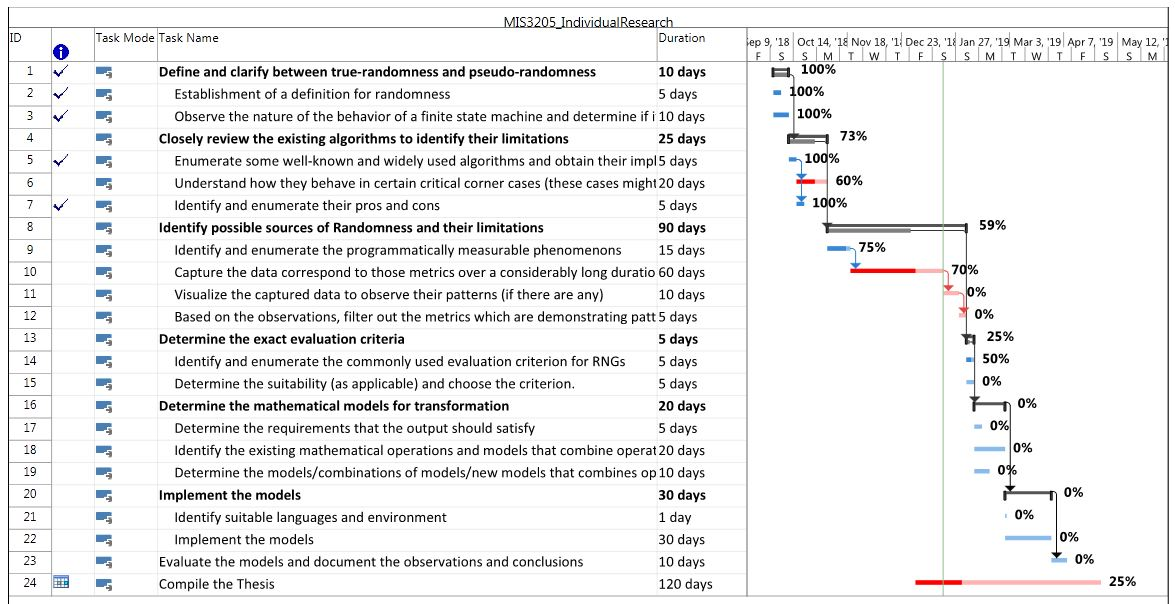
\includegraphics[width=1\textwidth, center]{images/wbs.JPG}
        \caption{Tracking Gantt Chart with Current Completion}
        \label{fig:track_gantt}
    \end{figure} \\
    
\newpage\section{Critical Review and Conclusion}
The important work items listed below, are currently behind schedule. It is required to devise a recovery plan expedite those tasks.
    \begin{enumerate}
        \item \ref{und_alg} Understanding the algorithms.
        \item \ref{capt_data} Capture intended data.
    \end{enumerate}
\par Developing the required routine has been a major challenge because there was a diverse range of environments and libraries to consider, causing information overload. Apart from that, choosing samples was a difficult matter, due to the lack of availability and accessibility. However these were worked out eventually.

\par It is required to commence the rest of the tasks swiftly. However, the impact of the delay is yet to be handled. Major constraint that restricts the progress is the time.

\par Knowledge acquisition on the existing algorithms and the technologies was at times difficult. That was again due to the lack of commitment, which is a consequence of the time constraint. It is important to get into decisions swiftly.

\par Certain important decisions are yet to be made on the following items of the WBS.
    \begin{enumerate}
        \item \ref{vis_data} Data visualization
        \item \ref{filter_met} Filtering of metrics
        \item \ref{id_math_models} Identify the suitable math models and combinations that could be used.
    \end{enumerate}

\par Also, justifying these choices and decision is also important. It is anticipated that these might consume a considerable amount of time.

\newpage
\bibliographystyle{IEEEannot}
\bibliography{ref}

\end{document}
